\chapter{Estado del arte}
\label{ch:estado-arte}

\section{Inteligencia artificial}

El campo de la inteligencia artificial en la actualidad se encuentra en un estado de rápida evolución, con una infinidad de usos que se extiende por una gran variedad de sectores económicos y sociales. Su capacidad para analizar y procesar grandes cantidades de datos o para mejorar la eficiencia en distintas industrias han hecho que se trate de una tecnología en auge. El estudio de McKinsey \& Company The state of AI in 2022 and a half decade in review estima que el 50\% de las empresas ya usan IA en sus tareas diarias, donde destacan la optimización de servicios, la creación de productos y el análisis del servicio al cliente.

El informe AI Index Report 2024 del Human-Centered AI Institute (HAI) de la Universidad de Stanford muestra que la IA ya supera a las habilidades humanas en ciertas tareas, como en la clasificación de imágenes, con una precisión del 97\% respecto al 95\% de los humanos, o en juegos, como el ajedrez, donde supera consistentemente a los jugadores humanos.

Aunque sin duda, el mayor crecimiento en los dos últimos años corresponde a las herramientas relacionas con la Inteligencia Artificial Generativa (IAG). Esta rama se centra en crear modelos capaces de generar contenido, como conversaciones, imágenes, videos o música. Aprende de datos ya existentes y produce nuevos con características similares. En este ámbito destaca la empresa OpenAI, que cuenta con ChatGPT, capaz de generar texto lógico y actuar como chatbot, o con Dall-E, que puede generar imágenes en base a la descripción que se entregue. The state of AI in 2023: Generative AI's breakout year, también de McKinsey \& Company, muestra que el 79\% de los encuestados dice haber tenido almenos alguna exposición a la IAG, lo que indica que es la herramienta de IA que más rápido está captando el interés del público general.

\begin{figure}[H]
    \centering
    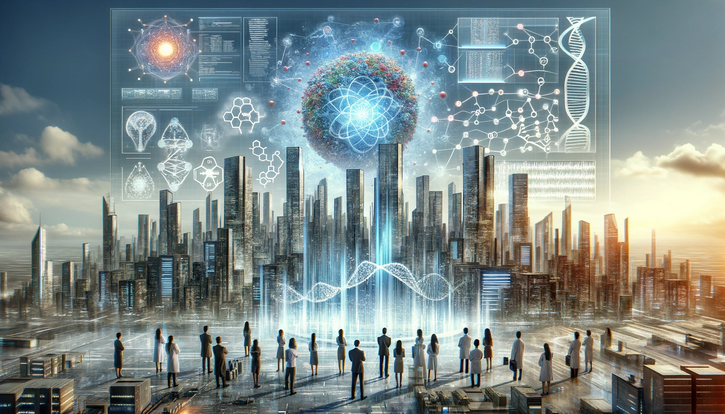
\includegraphics[width=0.5\textwidth]{figures/dall-e.png}
    \caption{Imagen generada con DALL-E 3.}
    \label{fig:dall-e}
\end{figure}

Existe una gran cantidad de proyectos pioneros actualmente relacionados con el campo de la IA. Algunos de los más importantes actualmente son:

\begin{itemize}
    \item AlphaFold. Este programa de Deepmind utiliza IA para predecir las estructuras de las proteínas. Ha permitido acelerar las investigaciones científicas que desembocan en la creación de nuevos medicamentos.
    \item Neuralink. Esta empresa trabaja en el desarrollo de un chip que permita comunicar directamente un cerebro humano con una computadora. Posibilitará realizar análisis neurológicos más precisos.
    \item Vehículos autónomos. Waymo controla una flota de taxis sin conductor que han estado operando por Estados Unidos. 
    \item Medicina personalizada. Análisis de datos genéticos y médicos para diseñar tratatamientos que sean más efectivos para el paciente.
\end{itemize}

\newpage

\section{Algoritmos evolutivos}

Los algoritmos evolutivos han tenido varios proyectos que han marcado el desarrollo de esta tecnología. Los primeros acercamientos tuvieron lugar en la década de 1960. Por un lado, Lawrence Fogel comenzó a explorar la programación evolutiva, centrándose en la evolución de autómatas finitos. Uno de los primeros intentos de aplicar principios evolutivos a la informática. Por otro lado, Rechenberg y Shwefel desarrollaron estrategias de evolución para problemas de optimización en ingeniería. Centradas en la selección y en la mutación, resultaron ser muy útiles para aplicarlas en la realidad.

Tras estos primeros pasos, John Holland fue fundamental para el desarrollo de los algoritmos genéticos. Su libro Adaptation in Natural and Artificial Systems del año 1975 es básico para entender el funcionamiento de los mismos. Su trabajo se centró en la idea de que la evolución biológica podía ser simulada y utilizada para resolver problemas complejos en computación. Hacen uso de los operadores como la selección, el cruce o la mutación para evolucionar una población candidata de individuos hacia una mejor solución. Cada solución es evaludada seguún una función de fitness, que mide qué tan buena es la solución al problema en cuestión.

\begin{lstlisting}[caption=Algoritmo Genético]
INICIAR
    INICIALIZAR población
    EVALUAR fitness
    REPETIR HASTA CUMPLIR condición de parada:
        SELECCIONAR individuos
        CRUZAR padres
        MUTAR hijos
        EVALUAR individuos
        FORMAR nueva generación
    RETORNAR solución
FINALIZAR
\end{lstlisting}

Después de que Holland sentara las bases de los algoritmos genéticos, en los años siguientes fueron surgiendo estudios que hicieron evolucionar la rama. Varios de los más importantes fueron de John Koza, quien introdujo la programación genética, técnica usada para desarrollar automáticamente programas que realicen una tarea definida por el usuario. Se optimiza una población de individuos (programas) respecto a una función de aptitud. Koza probó su viabilidad para resolver problemas de robótica o de optimización.

Tras él han seguido surgiendo nuevas técnicas dentro de los algoritmos evolutivos. Entre ellas se puede destacar el desarrollo de los Algoritmos genéticos híbridos (AGH), que combinan los algoritmos genéticos con otras técnicas de optimización para mejorar las soluciones a los problemas complejos. Otro avance importante es el de la Programación genética cartesiana (CGP), que sustituye los árboles de busca usados en la programación genética tradicional por grafos dirigidos, lo que es muy útil, por ejemplo, en el diseño de circuitos electrónicos.

A lo largo de los años se han desarrollado distintos proyectos pioneros que han hecho uso de los algoritmos genéticos. Algunos son:

\begin{itemize}
    \item Space Technology 5 (ST5). Se usó algoritmos genéticos para la creación de una antena ultracompacta para la misión ST5 de la NASA, superando las expectativas de rendimiento.
    \item The EvoTanks Project. Se estudió el uso de algoritmos genéticos para desarrollar estrategias de combate para tanques autónomos en simulaciones.
    \item Sector financiero. Se puede utilizar para predecir movimientos del mercado. Además, a nievel doméstico, hay apps que lo usan para optimizar el método de compartir gastos entre distintos usuarios.
    \item Bioingeniería. Ayudan a modelar secuencias genéticas, que acelera los avances en medocina personalizada.
\end{itemize}


\section{Planificación nutricional mediante algoritmos evolutivos}

Los primeros acercamientos para intentar resolver problemas de optimización nutricional se dan en la década de 1940. George Stigler, en su artículo The Cost of subsistence, planteó el problema de encontrar la dieta de menor coste que cumpliese con unos objetivos nutricionales. Al no poseer ordenadores, utilizó técnicas manuales.

El problema fue formalmente resuelto dos años después por Jack Laderman usando programación lineal. Fue capaz de calcular la combinación de alimentos que cumpliese con los requisitos económicos y nutricionales. Con esto se demostró la utilidad de técnicas computacionales en tareas de optimización.

Tras las bases que sentó Holland, empezaron a aparecer distintos trabajos que hacían uso de los algoritmos genéticos para resolver problemas de optimización, incluyendo los de planificación nutricional. Application of genetic algorithms to diet optimization problems por 








